\documentclass[modern]{aastex62}
\usepackage{amsmath}
\graphicspath{{./}{figures/}}

% typography
\setlength{\parindent}{1.\baselineskip}
\newcommand{\acronym}[1]{{\small{#1}}}
\newcommand{\project}[1]{\textsl{#1}}
\newcommand{\package}[1]{\textsl{#1}}
\newcommand{\gaia}{\textsl{Gaia}}
\newcommand{\pans}{\textsl{Pan-STARRS}}
\newcommand{\DR}[1]{\acronym{DR#1}}
\newcommand{\todo}[1]{{\color{red} TODO: #1}}

\newcommand{\articlename}{\textsl{Letter}}
\newcommand{\sectionname}{Section}

% astronomy stuffs
\newcommand{\msun}{\textrm{M}_\odot}
\newcommand{\kpc}{\textrm{kpc}}
\newcommand{\kms}{\ensuremath{\textrm{km}~\textrm{s}^{-1}}}
\newcommand{\bs}[1]{\boldsymbol{#1}}
\newcommand{\masyr}{\ensuremath{\textrm{mas}~\textrm{yr}^{-1}}}
\newcommand{\feh}{\ensuremath{[\textrm{Fe} / \textrm{H}]}}
%\newcommand{\kms}{\mbox{km s$^{-1}~$}}
\newcommand{\kmse}{\mbox{km s$^{-1}$}}
\newcommand{\vlsr}{$V_{\rm LSR}~$}
\newcommand{\vlsre}{$V_{\rm LSR}$}
\newcommand{\hi}{H{\footnotesize I} }
\newcommand{\hie}{H{\footnotesize I}}
\newcommand{\lms}{$L_{\rm MS}~$}
\newcommand{\lmse}{$L_{\rm MS}$}
\newcommand{\bms}{$B_{\rm MS}~$}
\newcommand{\bmse}{$B_{\rm MS}$}

\newcommand{\clustername}{\textsl{NAME}}
\newcommand{\lmcsmc}{LMC--SMC}

%% Reintroduced the \received and \accepted commands from AASTeX v5.2
% \received{January 1, 2018}
% \revised{January 7, 2018}
% \accepted{\today}

\submitjournal{ApJL}
\shorttitle{A recent star formation event in the Magellanic stream}
\shortauthors{Price-Whelan et al.}

\begin{document}

% \title{A young star cluster in the Galactic halo: \\
% Recent star formation associated with the Leading Arm of the Magellanic stream}
\title{A star formation event in the leading arm of the Magellanic stream triggered by passage through the outer Galactic disk}

\author[0000-0003-0872-7098]{Adrian~M.~Price-Whelan}
\affiliation{Department of Astrophysical Sciences,
             Princeton University, Princeton, NJ 08544, USA}
\email{adrn@astro.princeton.edu}
\correspondingauthor{Adrian M. Price-Whelan}

\author[0000-0002-1793-3689]{David L. Nidever}
\affiliation{Department of Physics, Montana State University, P.O. Box 173840, Bozeman, MT 59717-3840, USA}
\affiliation{National Optical Astronomy Observatory, 950 North Cherry Ave, Tucson, AZ 85719}

\author[0000-0003-1680-1884]{Yumi Choi}
\affiliation{Department of Physics, Montana State University, P.O. Box 173840, Bozeman, MT 59717-3840, USA}
\affiliation{Steward Observatory, University of Arizona, 933 North Cherry Avenue, Tucson AZ, 85721}

\author{Edward Schlafly}

\author{Douglas Finkbeiner}
% \affiliation{McWilliams Center for Cosmology, Department of Physics, Carnegie Mellon University, 5000 Forbes Avenue, Pittsburgh, PA 15213, USA}
% \affiliation{Institute of Astronomy, University of Cambridge, Madingley Road, Cambridge CB3 0HA, UK}

\author{Sergey E. Koposov}
\affiliation{McWilliams Center for Cosmology, Department of Physics, Carnegie Mellon University, 5000 Forbes Avenue, Pittsburgh, PA 15213, USA}
\affiliation{Institute of Astronomy, University of Cambridge, Madingley Road, Cambridge CB3 0HA, UK}

\author{Vasily Belokurov}
\affiliation{Institute of Astronomy, University of Cambridge, Madingley Road, Cambridge CB3 0HA, UK}
\affiliation{Center for Computational Astrophysics, Flatiron Institute, 162 5th Avenue, New York, NY 10010, USA}


\begin{abstract}

We report the discovery of a young ($\lesssim 100~\textrm{Myr}$), metal-poor ($[\textrm{Fe}/\textrm{H}] \sim -1$) stellar association in the halo of the Milky Way ($(R, z) \sim (24, 16) kpc$).
The association --- \clustername\ --- is likely associated with the leading arm of the gas stream emanating from the Magellanic cloud system, but is located $\approx 60^\circ$ from the Large Magellanic Cloud (LMC) center, on the other side of the Milky Way disk relative to the LMC.
By assuming that the cluster is co-located with HI gas in the stream, we directly measure the distance to the Magellanic stream, $d \approx 25~\textrm{kpc}$.
At this location relative to the LMC, the measured distance is inconsistent with predictions from models of the LMC/SMC interaction and infall into the Milky Way. \todo{that don't account for ram pressure and gas interaction with MW disk}
The estimated age of \clustername\ is consistent with the time of last passage through the Galactic midplane.
We therefore conclude that this star-formation event was triggered by the last disk passage, which occurred at a Galactocentric radius $R \approx XX~\kpc$.

\end{abstract}

\keywords{Galaxy: halo}


\section{Introduction} \label{sec:intro}

The halo of the Milky Way is characterized by its old ($\gtrsim 10~\textrm{Gyr}$), metal-poor ($\feh \approx -1.5$) stellar population.
This is understood as a signature of the dominant (in stellar mass) progenitor systems that were accreted and disrupted early on in the formation of the Galaxy: massive dwarf galaxies \citep[e.g.,][]{Deason:2015, Fiorentino:2015}.
These systems likely came in with significant gas reservoirs, but were quenched and stripped through collisional processes that heated and dispersed the gas \citep[e.g.,][]{Mayer:2006}, thus preventing immediate star formation in the deposited gas.
The Milky Way, however, continues to accrete satellite galaxies, as is evidenced by the prominent stellar stream from the Sagittarius dwarf galaxy \citep{Ibata:1994, Majewski:2003}, and the presence of the Large and Small Magellanic Clouds (LMC, SMC) within the virial radius of the Galaxy.
While Sagittarius was likely stripped of its neutral gas long ago \citep{Burton:1999, Tepper-Garcia:2018}, the \lmcsmc\ system is associated with $\approx 8\times 10^8~\msun$ of HI gas \citep{Bruns:2005}, which extends into leading and trailing gas streams that wrap nearly $\approx 200^\circ$ around the sky \citep{Putman:1998, Bruns:2005, Nidever:2010}.

The Magellanic stream (MS) is a large stream of (predominantly) hydrogen gas emanating from the \lmcsmc\ system that contains a significant fraction of the total gas mass associated with the \lmcsmc\ \citep{Bruns:2005}.
The stream was discovered in early surveys of 21 cm emission and has since been studied in great detail by large-area radio sky surveys, and in H$\alpha$ emission \citep{Weiner:1996, Barger:2017}.
With increased resolution, surveys have found small-scale structure and gas fragmentation \citep[e.g.,][]{Nidever:2008, For:2014} and a large-scale bifurcation, with semi-distinct ``strands'' that lead back to the LMC and broader system, respectively \citep[e.g.,][]{Morras:1983, Putman:2003}.
As surveys push deeper to lower column densities, extensions of the stream have been found both in the trailing region \citep{Nidever:2010}, but also in the leading arm, which has been found to connect to regions of low-column-density gas ($N\sim 10^{18}$--$10^{19}~\textrm{cm}^{-2}$) on the other side of the Galactic disk \citep{Putman:1998, Nidever:2008}.
The leading arm (LA) has been decomposed into three or four distinct ``features'' named LA1--4 \citep{Bruns:2005, Nidever:2008, Venzmer:2012} with total HI mass $\sim 4 \times10^7~\msun$ \citep{Venzmer:2012}.

The origin and formation of the LA features in the MS is still uncertain.
Initial studies of the LA argue that the features closest to the \lmcsmc\ can be traced back to the SMC, thus implying that the gas in the LA was stripped from the SMC \citep{Putman:1998}.
In more recent work, it has instead been argued that outer features of the LMC appear to lead directly into the LA-1 feature \citep{Nidever:2008}, implying an LMC origin for the leading arm.
Whatever the origin of the gas, it is clear that tidal stripping by the Milky Way is required to form the leading arm \citep{Nidever:2008}.
However, the LA features deviate from the predicted orbit of the \lmcsmc, implying that ram pressure or interactions with gas in the outer Milky Way disk may have removed orbital energy from the LA gas \citep[e.g.,][]{Bekki:2008}.

Streams formed from tidally stripped material --- such as the Sagittarius or Palomar 5 \citep{Odenkirchen:2001} stellar streams, or gas streams such as the MS --- encode information about the orbital history and future trajectory of their progenitor system \citep[e.g.,][]{Johnston:1999}.
For this reason, streams of debris are of interest for constraining the dark matter distribution around the Galaxy, as well as for providing a fossil record of the Milky Way's accretion history \citep{Johnston:1998, Bullock:2005}.
Several groups have attempted to use the MS to constrain both the infall history of the \lmcsmc\ and the dark matter halo of the Milky Way (see recent review by \citealt{DOnghia:2016}).
Early models for the formation of the MS invoke ram pressure and tidal stripping to explain the sky distribution and extent of the MS, and typically require that the \lmcsmc\ system complete several orbits around the Galaxy in order to strip enough material \citep[e.g.,][]{Murai:1980, Gardiner:1994, Mastropietro:2005}.
However, later measurements of the proper motion of the LMC (\citealt{Kallivayalil:2006}, later confirmed by \gaia\ \citealt{van-der-Marel:2016}) and improved models for the infall dynamics \citep{Besla:2007} suggest instead that the \lmcsmc\ system could be on its first passage through the Galaxy \citep{Besla:2010, Besla:2012}.
In addition, the orbit of the LMC implied by the new proper motion measurement appears to be offset by $\approx 10^\circ$ from the trailing MS \citep{Besla:2010}.
Put together, these recent revelations have led to new models for the formation of the MS that largely rely on past interactions between the LMC and SMC to preprocess the gas distribution before infall and eventual stripping by the tidal field of the Milky Way \citep{Besla:2012, Diaz:2012}.

One critical difficulty in using the MS to constrain models of the \lmcsmc\ interaction and infall is the lack of distance information along the stream.
No significant over-density of stars have been found associated with the trailing portion of the MS \citep{Guhathakurta:1998}, thus leaving distance and tangential velocity information largely unknown.
Recently, a small number of young OB stars have been found in the vicinity of the leading arm gas, with radial velocities consistent with having formed from the leading MS \citep{Casetti-Dinescu:2014, Zhang:2017}.
However, given their sparsity and concentration near the Galactic plane, it is difficult to unambiguously associate them with the MS: these could instead be runaway OB stars from the Milky Way disk.

In this \articlename, we report the discovery of a clustered association of young stars at the far edge of the LA-2 feature ($L_{\textrm{MS}} \sim 65^\circ$) that is unambiguously located far into the Galactic halo ($d_\odot \sim 30~\textrm{kpc}$) and therefore likely formed from gas in the leading arm of the Magellanic stream as it crossed the Galactic disk.
This provides a clear distance measurement to the leading arm of the MS to be compared with models of \lmcsmc\ interaction and infall into the Milky Way.

In \sectionname~\ref{sec:data}, we present the initial discovery with \gaia\ \DR{2} and follow-up observations with DECam to obtain deeper photometry of the region around the association.
In \sectionname~\ref{sec:results}, we derive estimates for the total stellar mass of, age of, and distance to the association, and present a plausible formation scenario.
In \sectionname~\ref{sec:discussion}, we discuss implications for future searches for stars associated with the MS, and discrepancies with existing models of the LA.
We conclude in \sectionname~\ref{sec:conclusion}.

\section{Data and cluster discovery} \label{sec:data}

We use astrometric data from the \gaia\ mission (\citealt{Prusti:2016}), data release 2 (\DR{2}; \citealt{Gaia-Collaboration:2018, Lindegren:2018}) to search for distant, comoving multiplets of blue stars.
We initially select all stars from \gaia\ with $\textrm{parallax} < 1$, $-0.5 < \bprp < 0$, $G < 20$, and Galactic latitude $|b| > 20^\circ$ (see Appendix~\ref{sec:queries} for database query).
We further exclude stars within a $15^\circ$ radius from the LMC, and a $8^\circ$ radius from the SMC --- this leaves just 27,895 stars.
We then cross-match this catalog to itself with both sky positions and proper motions: we search for pairs of stars that have separations $s < 0.5^\circ$ and proper motion differences $|\Delta \mu| < 0.5~\masyr$.
We then combine mutually-connected comoving pairs into small groups of stars that are colocated on the sky and comoving in proper motions; We filter out groups that have $<4$ members.
We cross-match the mean sky positions of the groups to locations of local group galaxies \todo{citation} \citep{Mcconaghie} and Milky Way globular clusters \todo{citation} \citep{Harris} and filter out all groups that lie within 1 degree of these known objects.
After these filters, just one group of blue, comoving stars remains at $(\textrm{RA}, \textrm{Dec}) \sim (179, -29)^\circ$.

We then query all objects from the \gaia\ \DR{2} catalog within a polygon centered on the nominal position of the group (see above), with a width of $12^\circ$ and a height of $8^\circ$ in the Magellanic stream coordinate system \citep{Nidever:2008} (see Appendix~\ref{sec:queries} for the database query).
We cross-match the resulting catalog with \acronym{GALEX} \todo{citation} using a positional crossmatch requiring source separation $<2~\textrm{arcsec}$, and with \acronym{PS1} \todo{citation}\citep{Chambers:XX} using the cross-match provided by the \gaia\ science archive.
\figurename~\ref{fig:cmds} shows a few color-magnitude and color-color diagrams from the cross-matched photometry, with magnitudes corrected for dust extinction using the SFD \citep{Schlegel:1998} dust map.

\todo{Left off here}

Figure \ref{fig_skypm} shows the spatial and proper motion distribution in the region of interest with the objects in
a small proper motion selection shown as black and red dots.  The color magnitude diagram (CMD) of the same objects
is shown in Figure \ref{fig_cmd} and clearly reveals a sequence of objects that follow the shape of a young main-sequence.
The PS1 photometry of the same region is shown in Figure \ref{fig_isochrone} and as well as young, metal-poor isochrones at fa distance of 25 kpc.  Finally, Figure \ref{fig_gass} shows a position-velocity diagram at the position of the cluster of the \citep[GASS;][]{McClure-Griffiths:2009} \hi data that has been Gaussian decomposed using the technique in \citet{Nidever:2008}.
The component of the LA II can be seen on the left-hand side of the figure and a similar \hie stream can be seen near the
position of the cluster.
% Yumi:
% Need a sentence or two for dust extinction correction somewhere in the above two paragraphs?

Isochrone: \citep{Fox:2018}


\section{Results} \label{sec:results}

We have used the new Gaia data to detect a young, metal-poor cluster in the halo of the Milky Way at a distance of 25 kpc and a MW z-height of 12 kpc.  The detection of such a young cluster so far from the star-forming disks of any nearby
galaxy is highly unusual.  However, the proximity of the new cluster to the Leading Arm of the Magellanic Stream suggests
that the cluster originated from this metal-poor gas \citep{Fox:2018}.  Previously studies have detected young stars in the Leading Arm and gas in the periphery of the Magellanic Clouds \citep{Casetti-Dinescu:2014, MoniBidin:2017}, however, this is the first time that an entire star cluster has been detected so far from the Clouds.

We evaluate the hypothesis that the cluster formed in the Leading Arm.  The mean proper motion values in the Magellanic Stream coordinate system \citep{Nidever:2008} are ($\mu_{\rm MSL}$,$\mu_{\rm MSB}$)=($+$1.X,0.X) mas yr$^{-1}$ which is very similar to the mean values of the LMC and SMC with ($+$1.X,0.X) mas yr$^{-1}$ and ($+$1.X,0.X) mas yr$^{-1}$, respectively.  The simulations of \citet{Besla:2012} also predict proper motions at this position of approximately ($+$1.X,0.X) mas yr$^{-1}$.  The Magellanic Stream simulations give distances of the Leading Arm at this position of $\sim$50 kpc, however, many of these do not include the effects of ram pressure from the hot MW halo which could cause the gas to drop in its orbit to smaller Galactocentric distances (NEED TO DOUBLE-CHECK THIS).  In addition Figure \ref{fig_gass} shows that there is Leading Arm \hi~gas at the position of the position of the cluster with a velocity of \vlsr=70 \kmse.



\begin{figure}
\centering
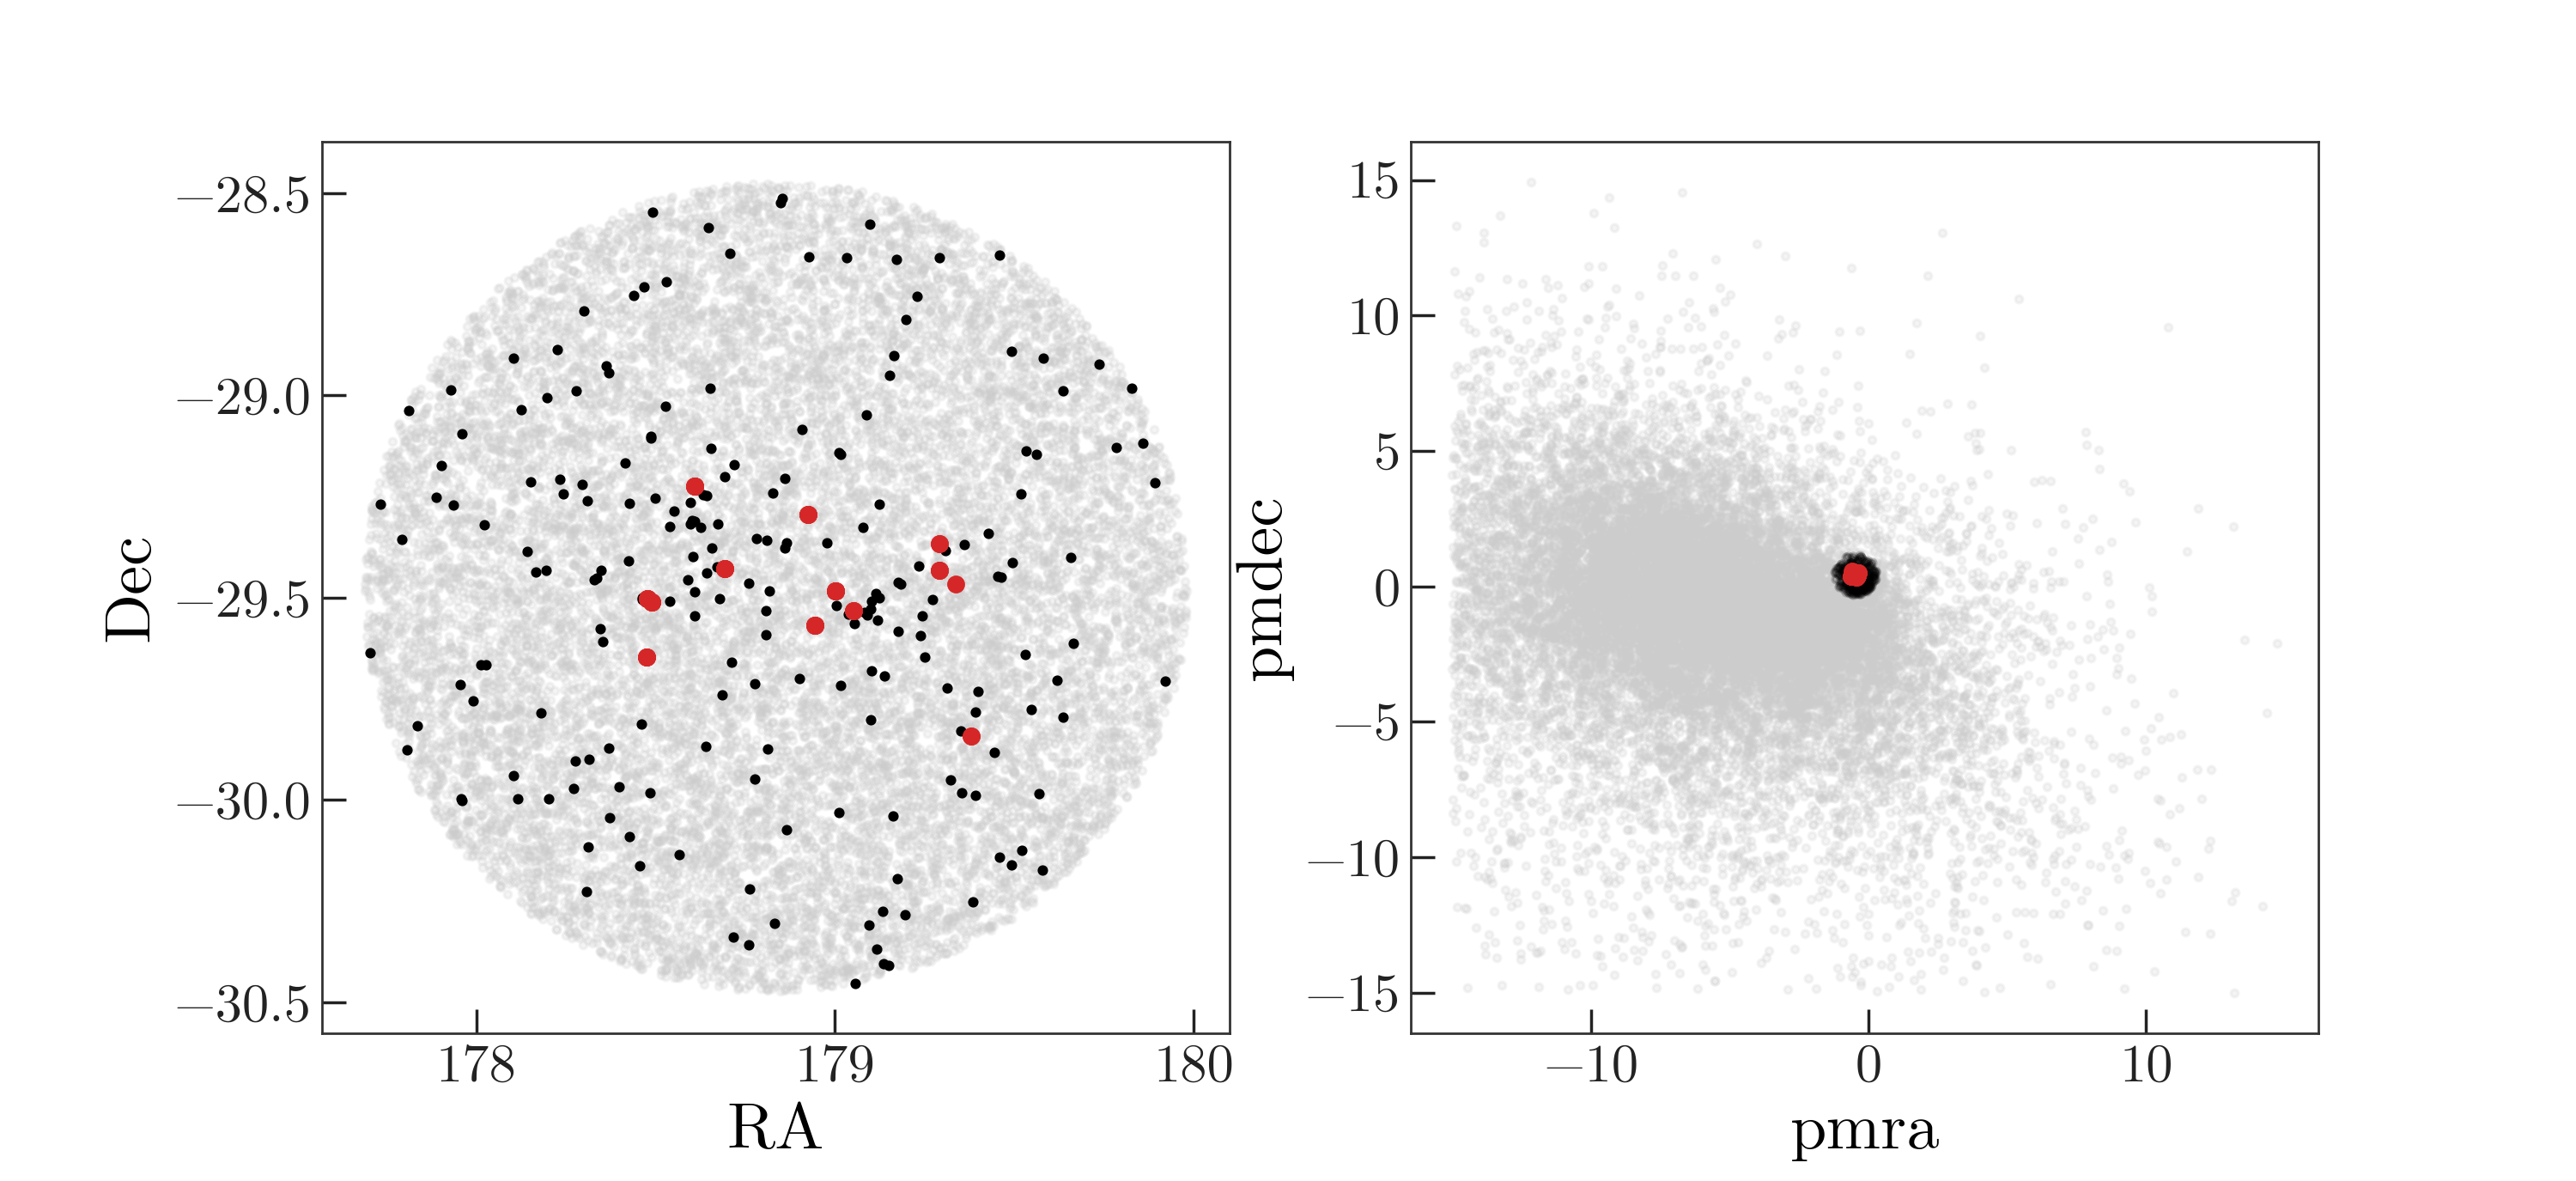
\includegraphics[width=12cm]{sky_pm.png}
\caption{Figure 1}
\label{fig_skypm}
\end{figure}

\begin{figure}
\centering
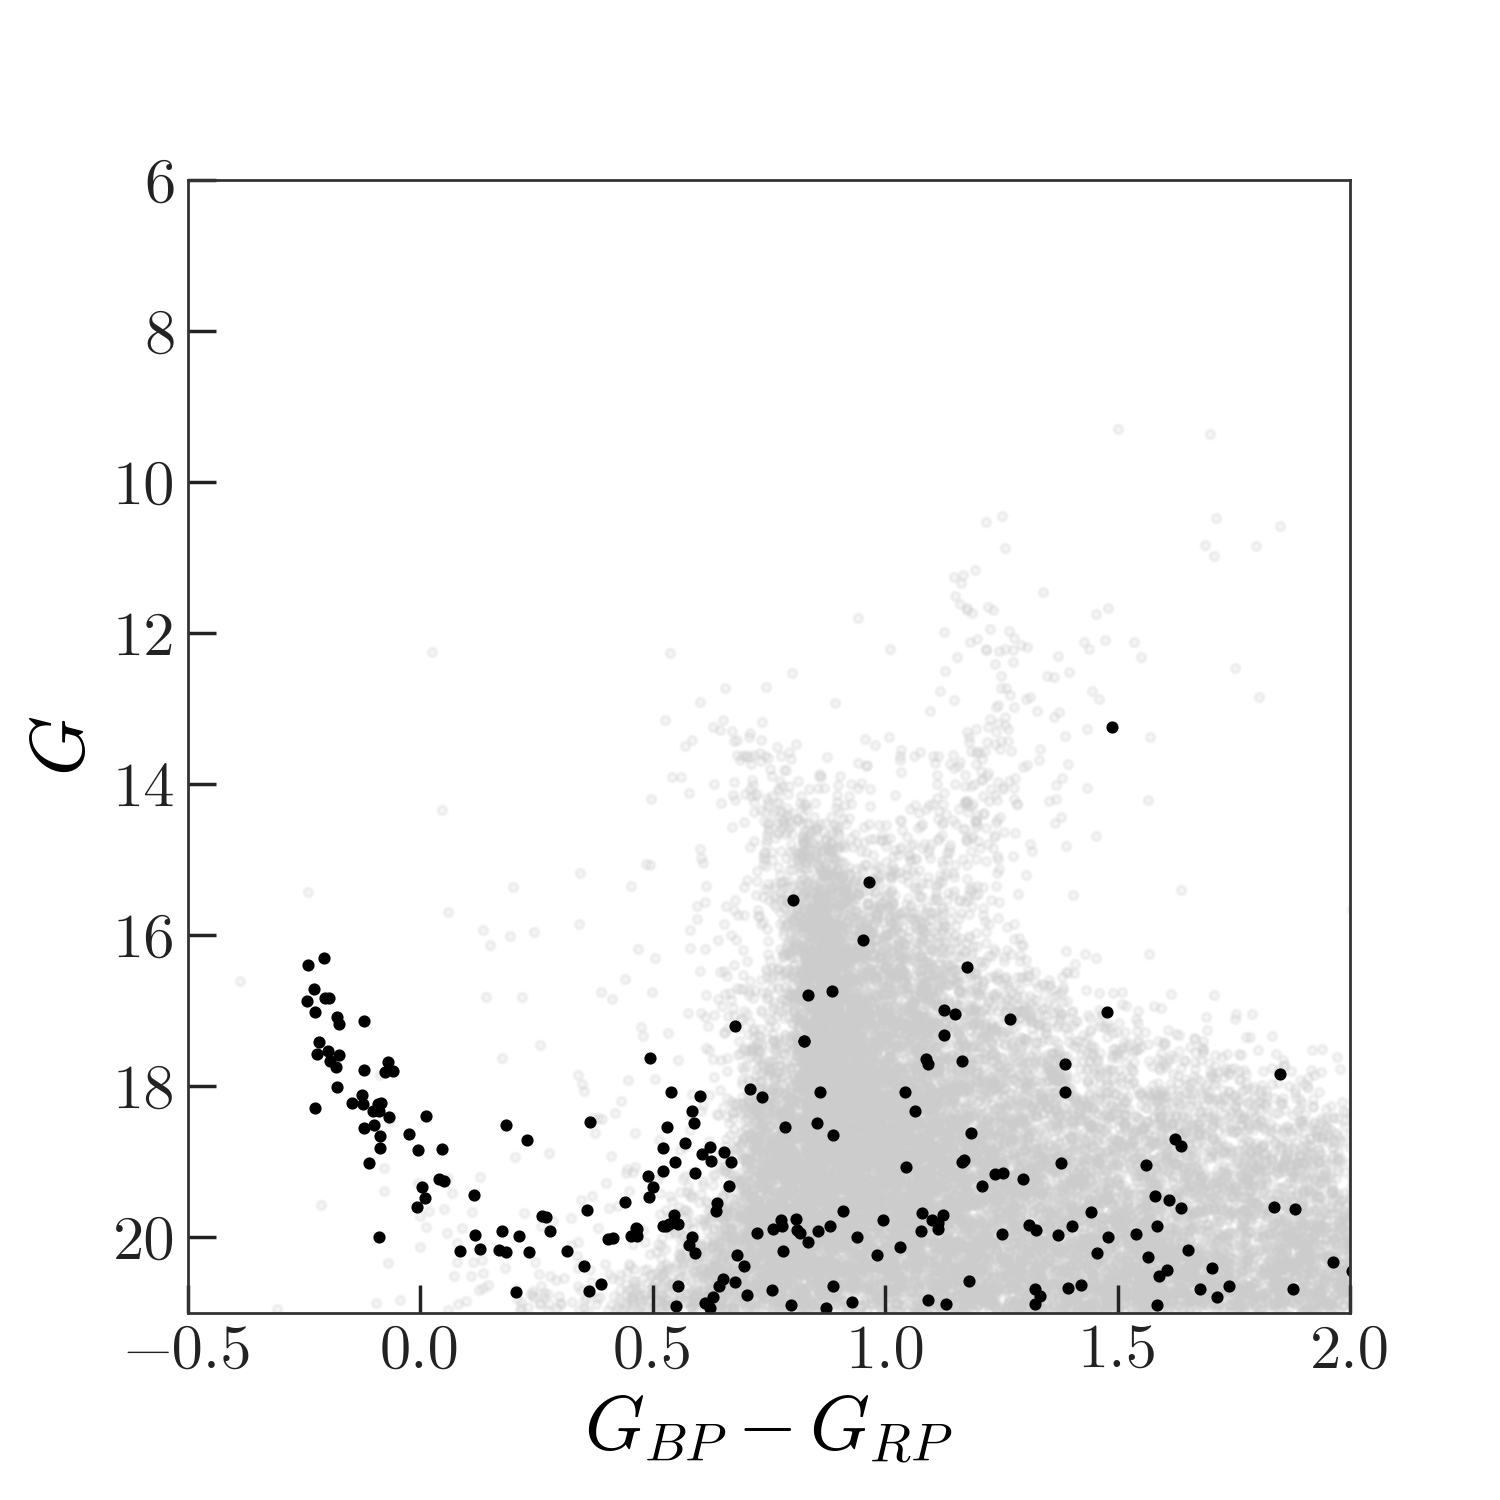
\includegraphics[width=8cm]{cmd.png}
\caption{The Gaia DR2 color magnitude diagram of the region showing the pronounced
young stellar main sequence.}
\label{fig_cmd}
\end{figure}

\begin{figure}
\centering
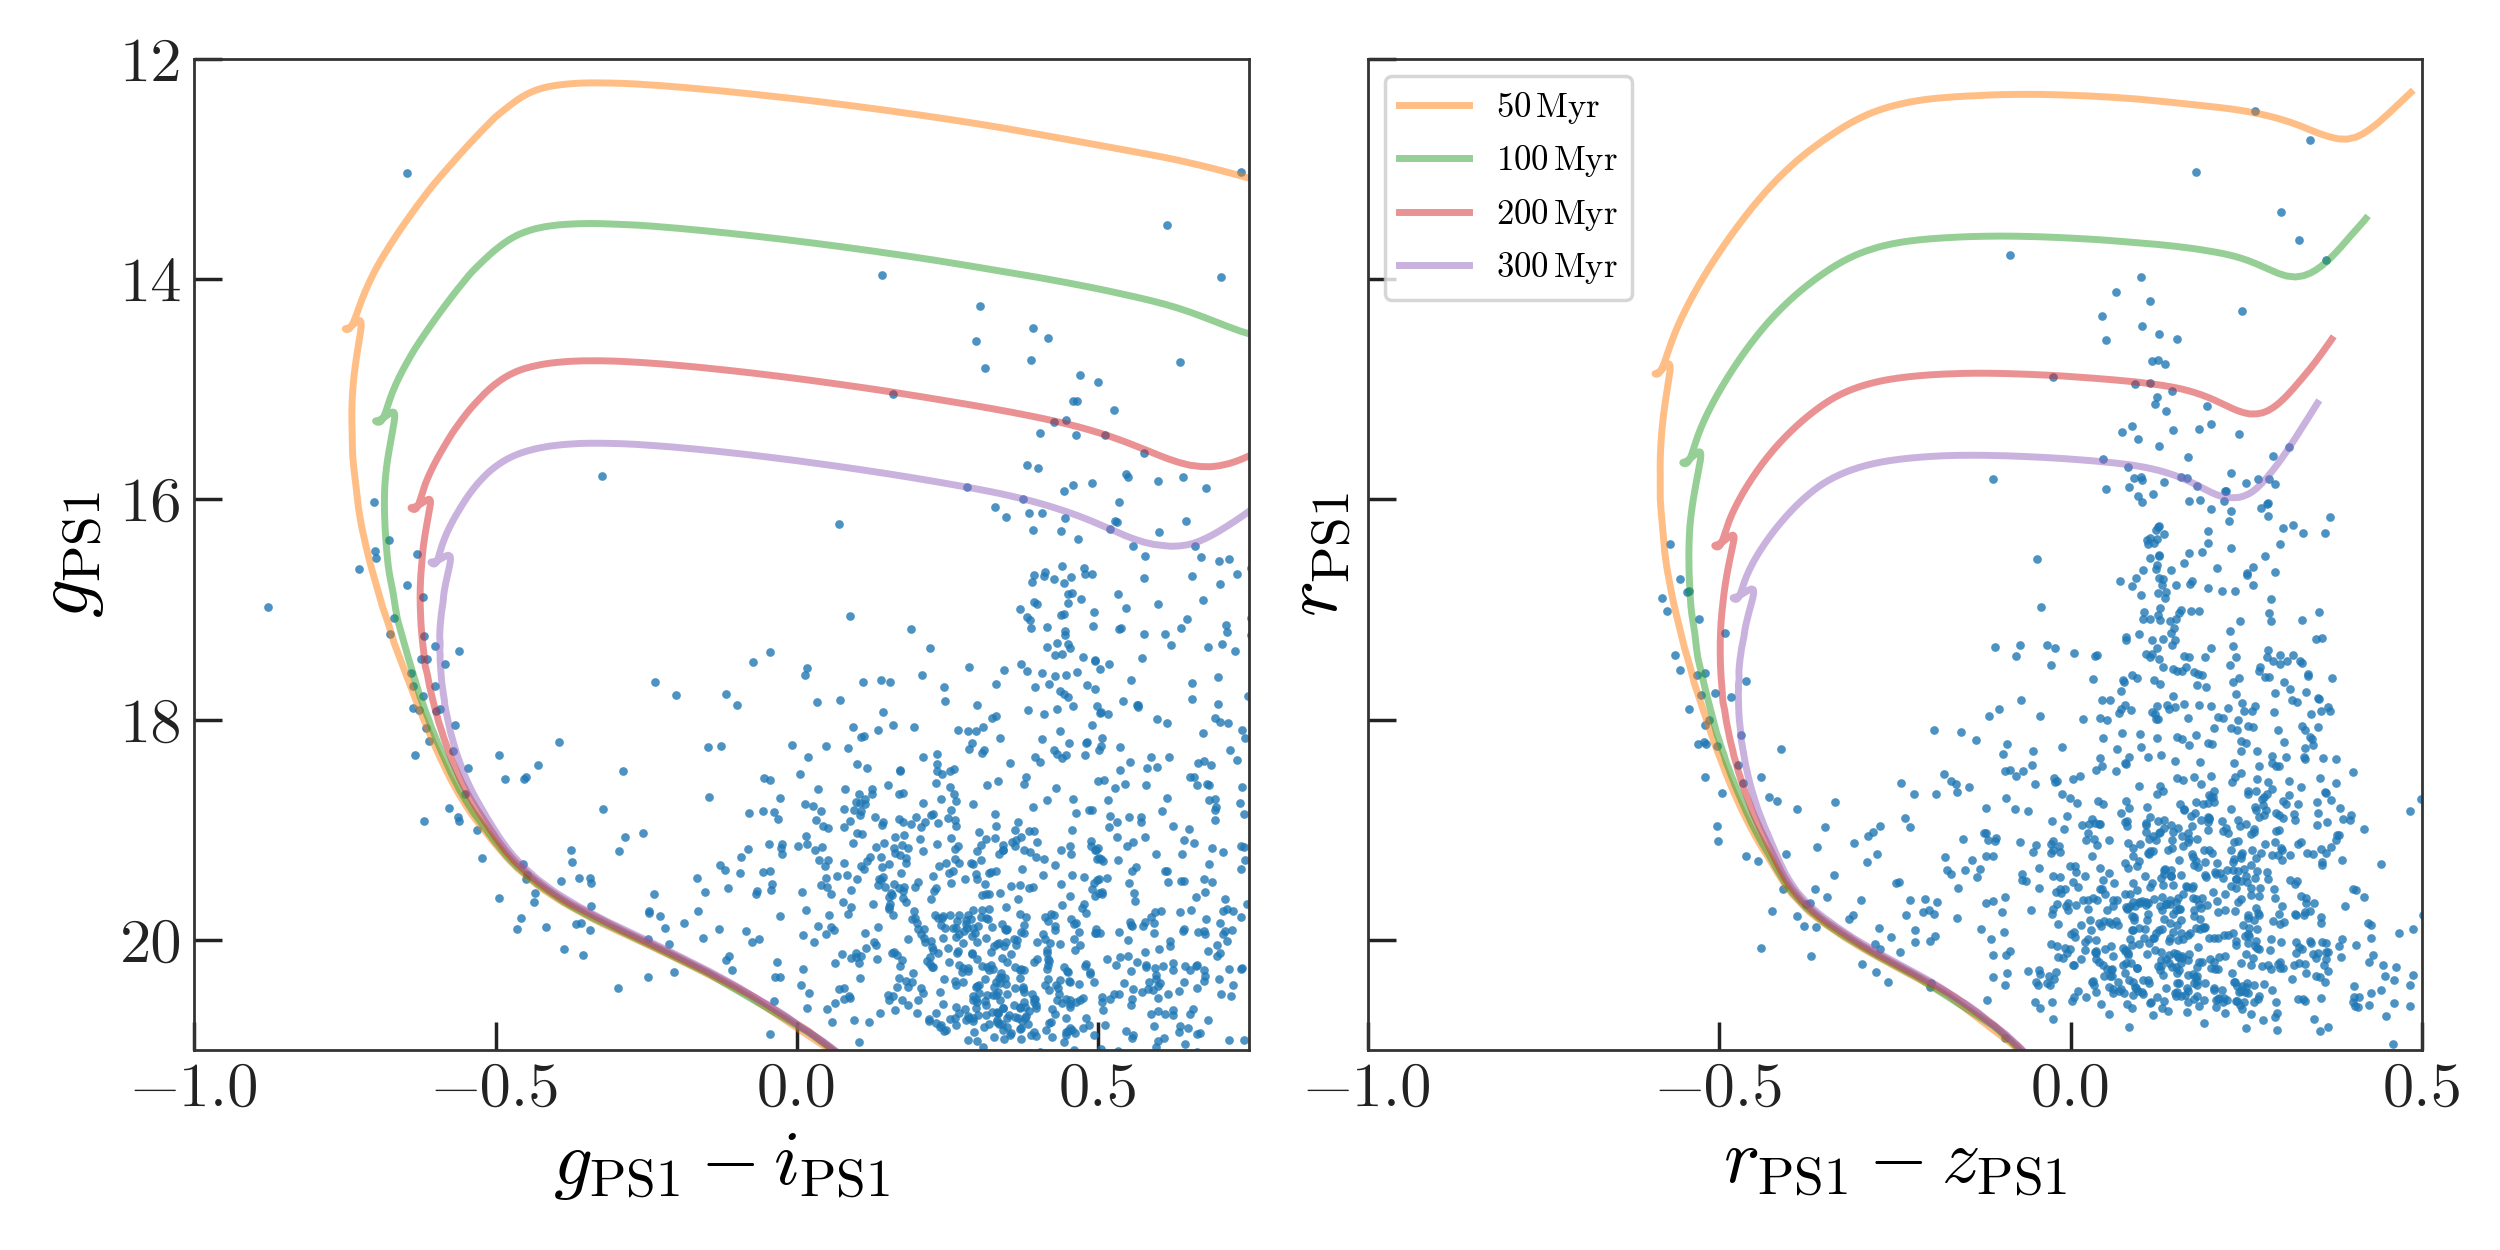
\includegraphics[width=8cm]{isochrone.png}
\caption{PS1 color magnitude diagrams with young, metal-poor (\feh=-1.0) isochrones overplotted at
a distance of 25 kpc.}
\label{fig_isochrone}
\end{figure}

\begin{figure}
\centering
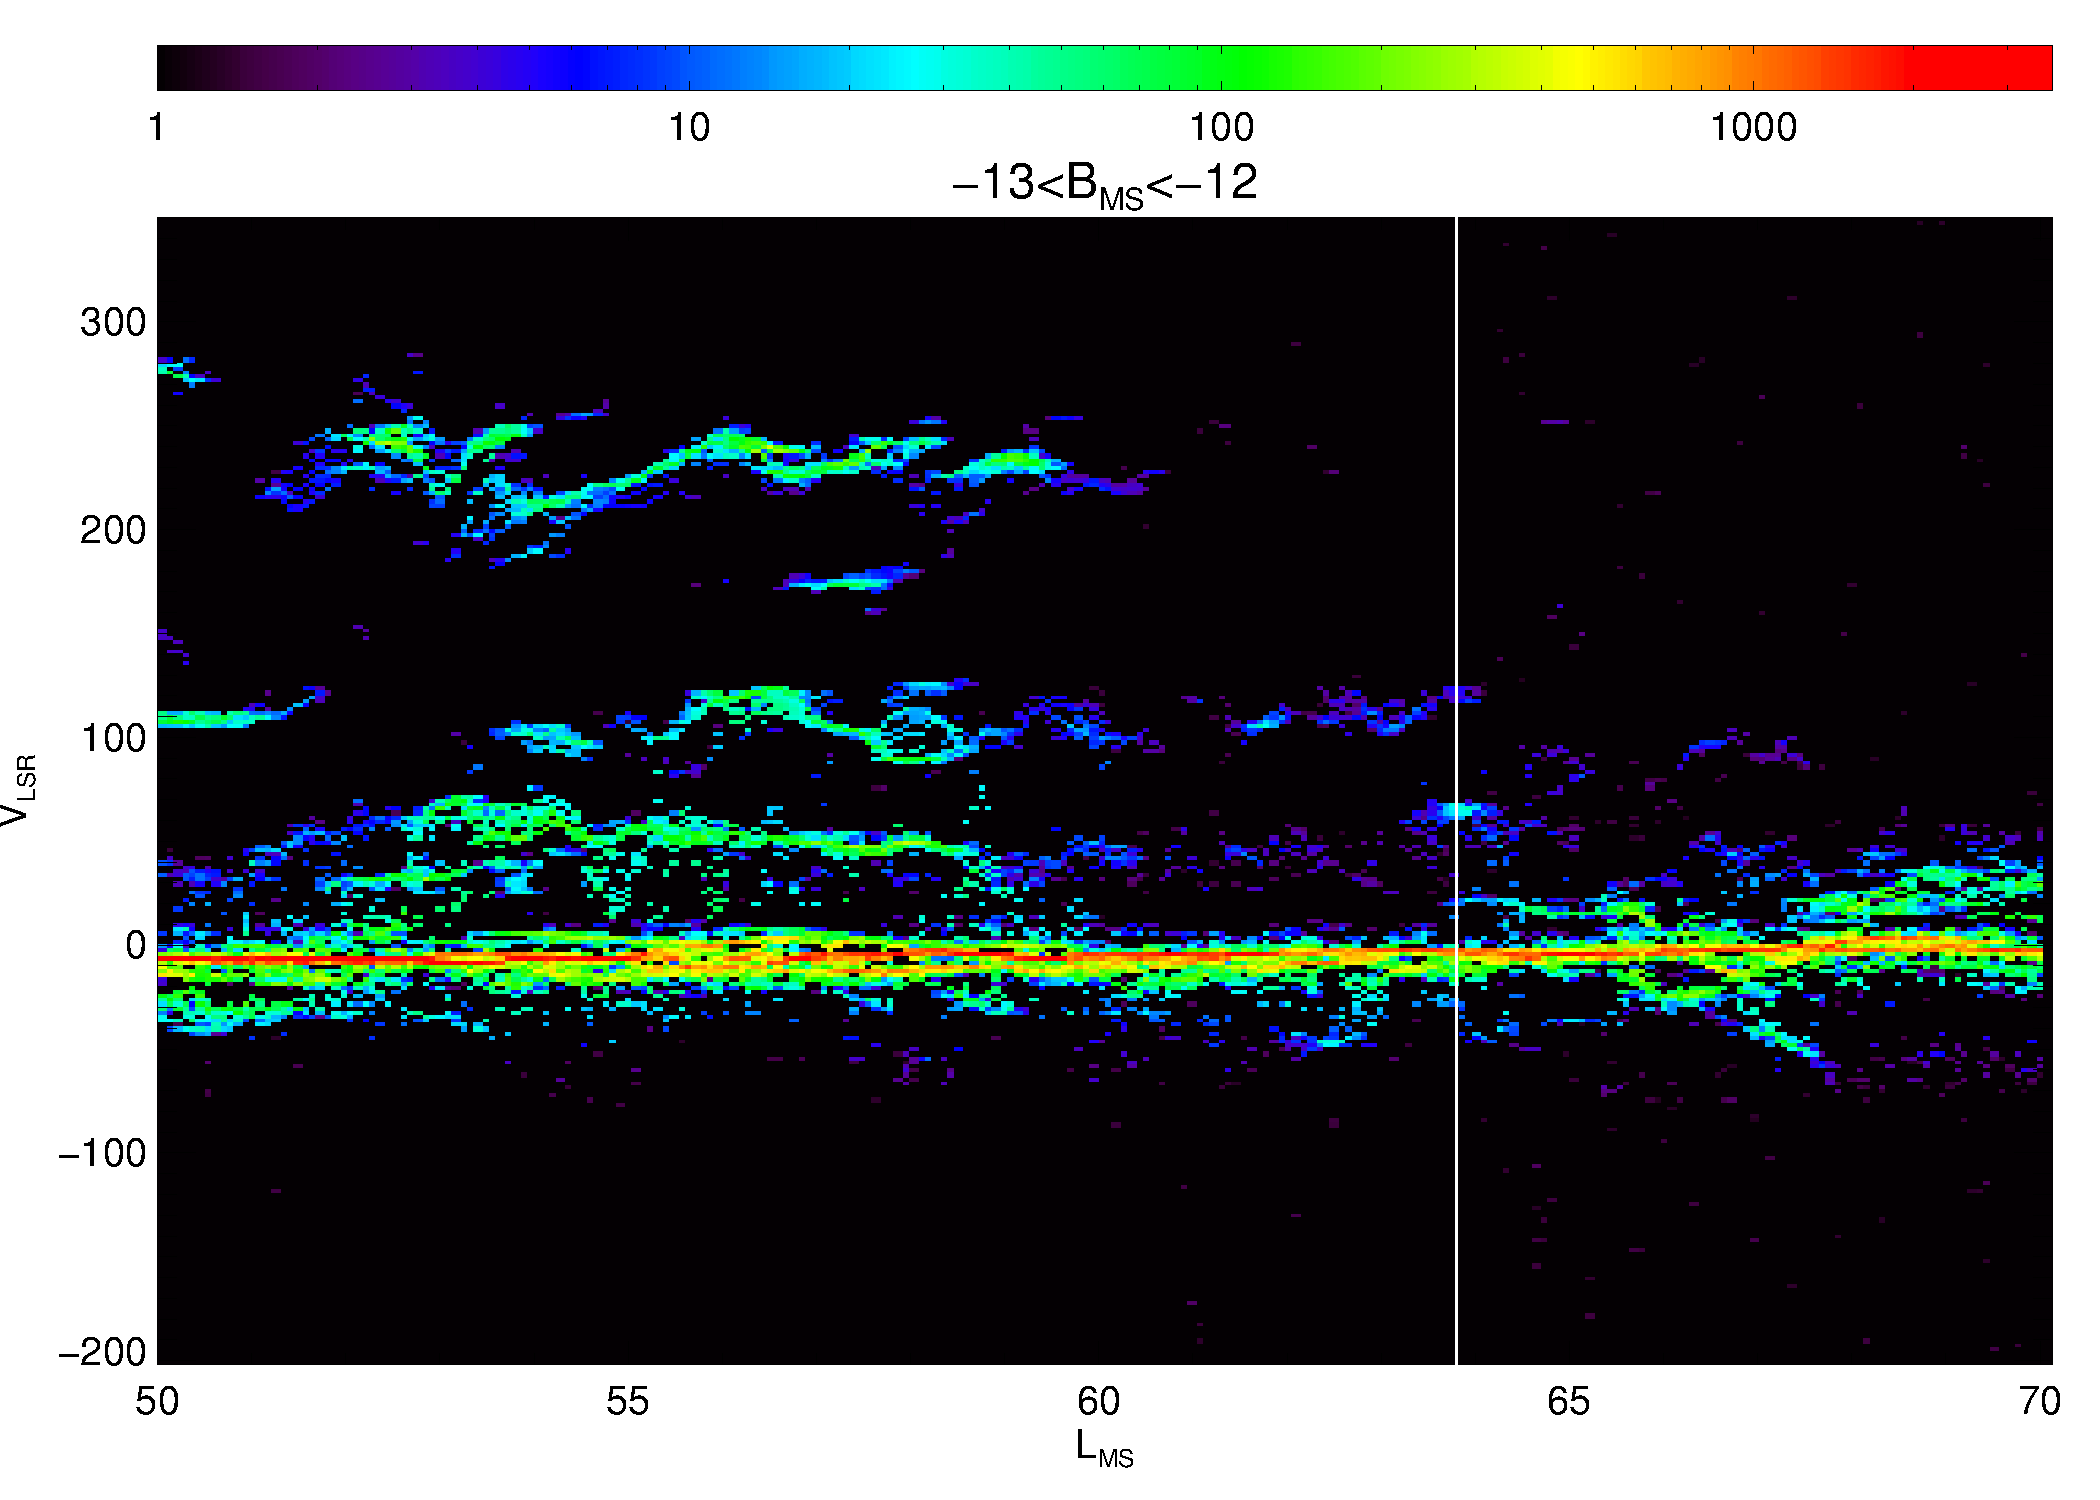
\includegraphics[width=8cm]{gass_vlsrmlon.pdf}
\caption{GASS position-velocity diagram.}
\label{fig_gass}
\end{figure}

\begin{figure}
\centering
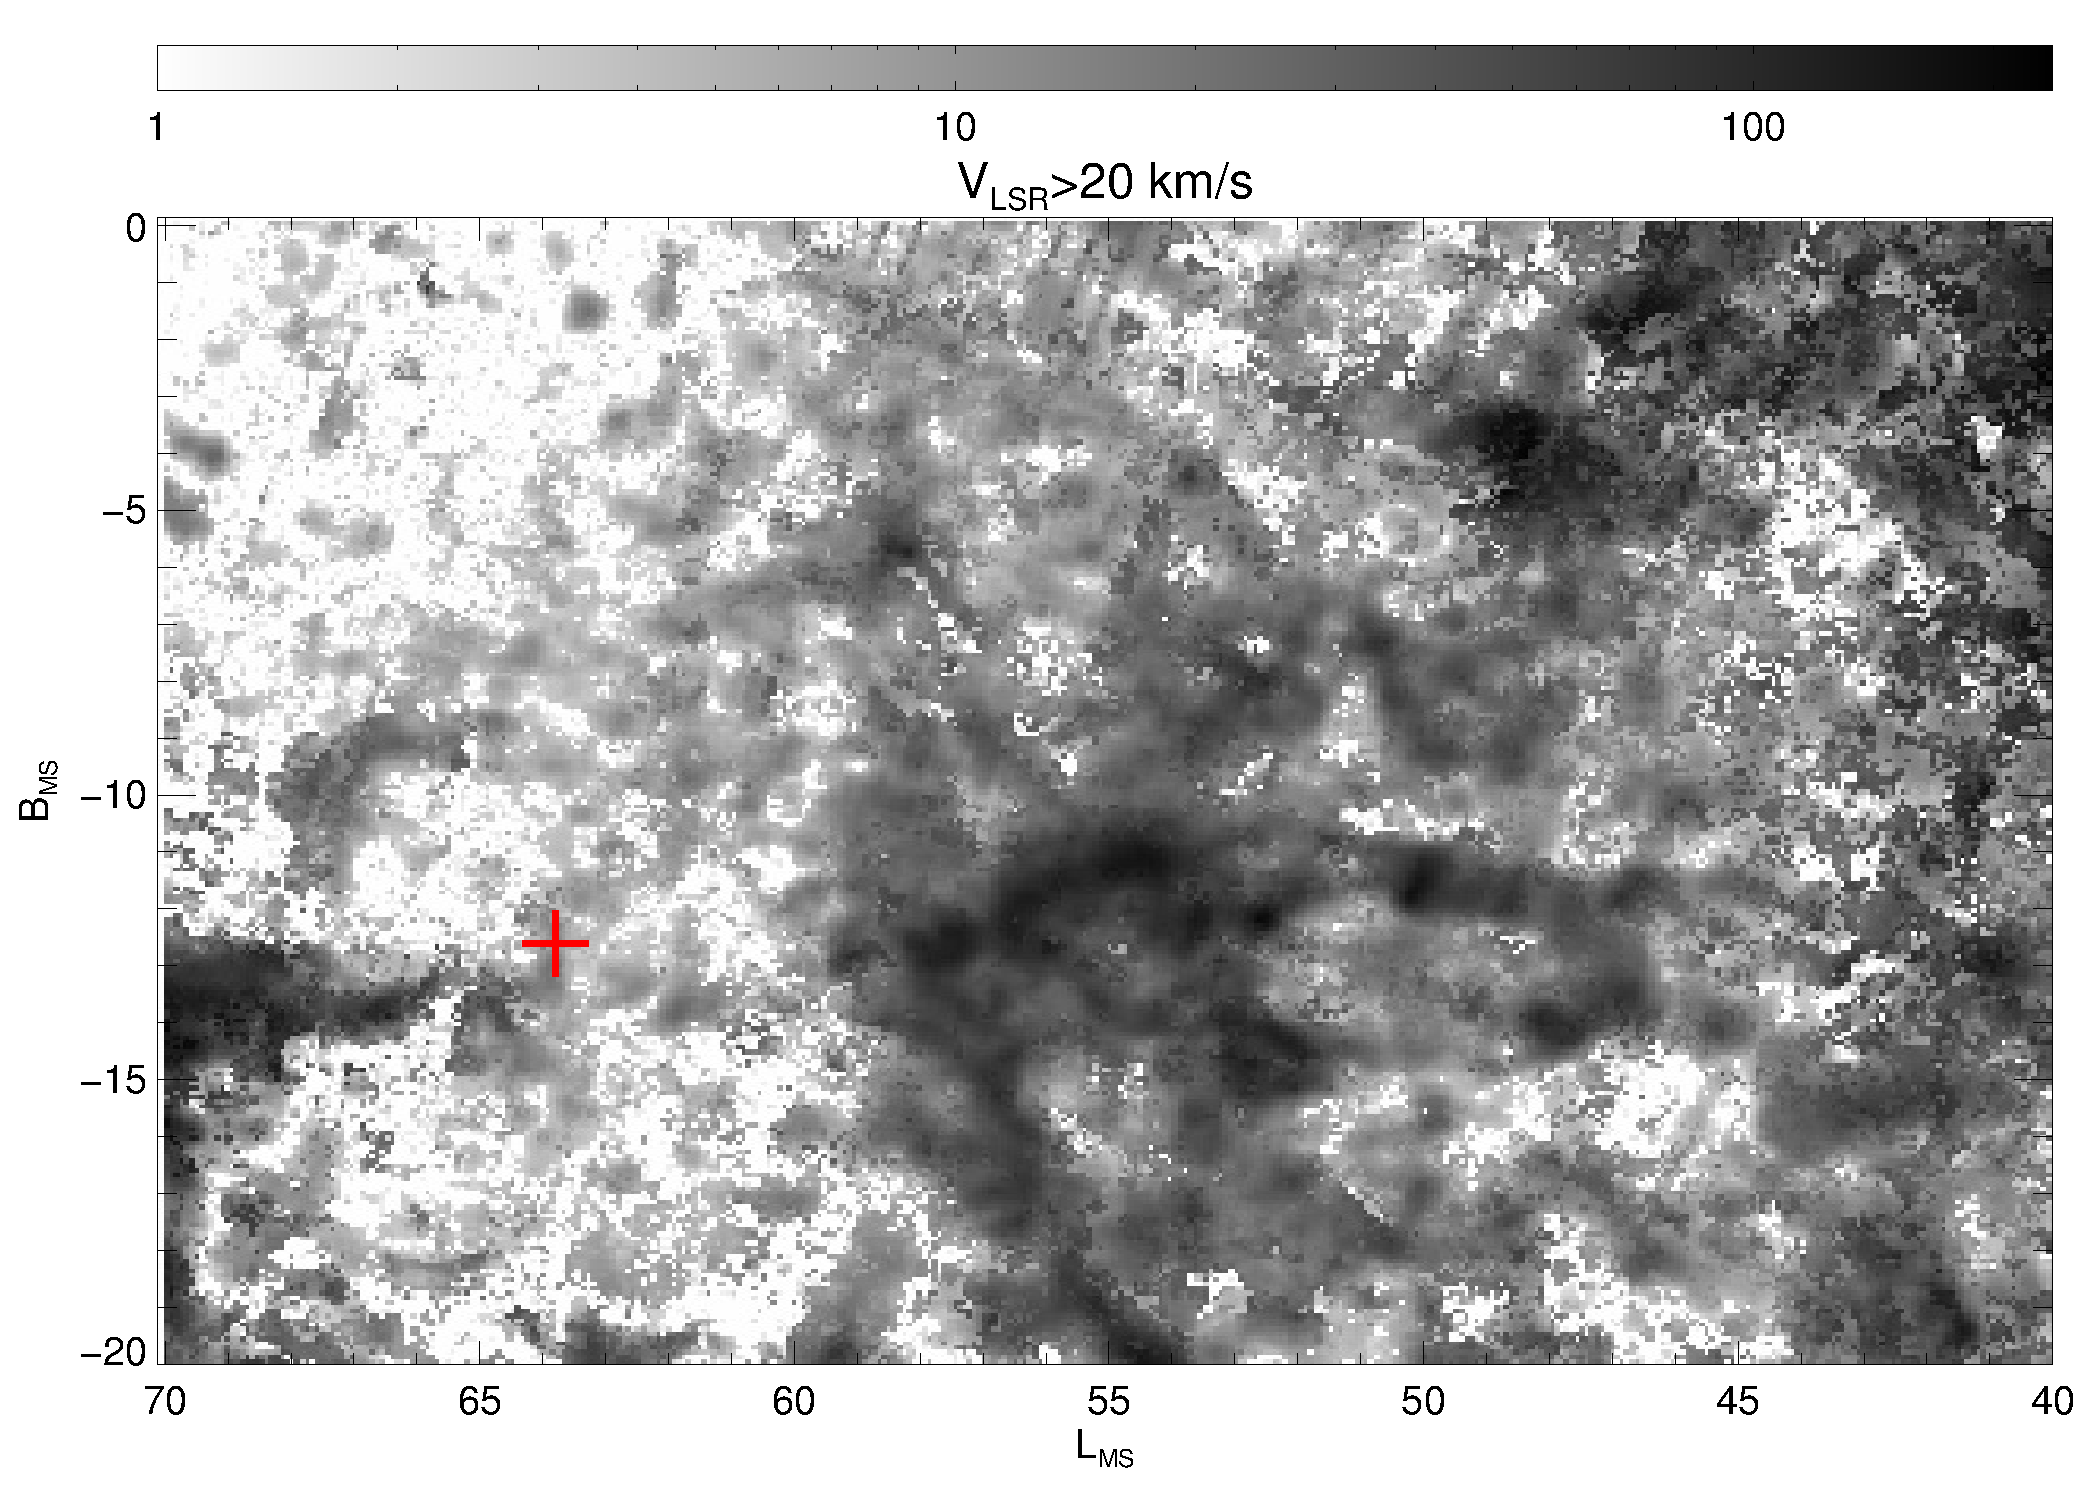
\includegraphics[width=8cm]{gass_mlatmlon.pdf}
\caption{GASS \hi column density in the region of LA II. The red cross marks the position
of the young cluster.}
\label{fig_gass}
\end{figure}

\begin{figure}
\centering
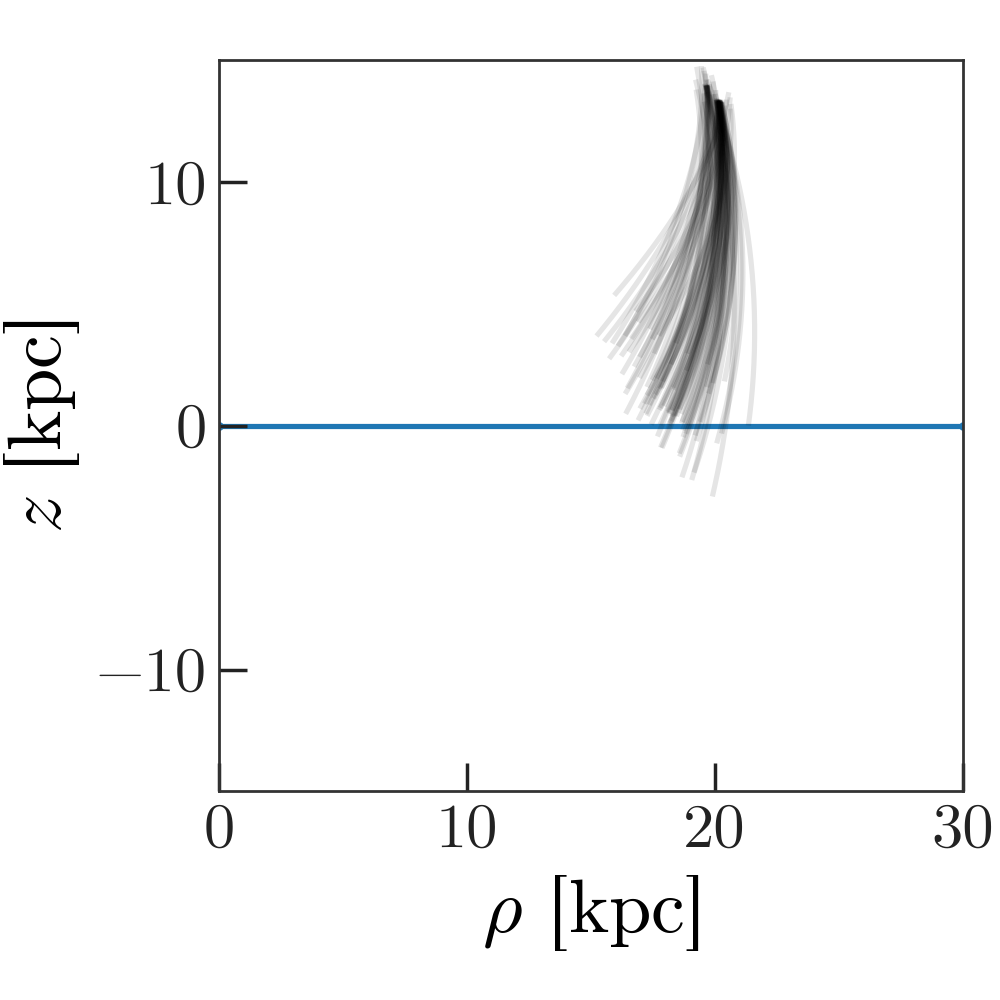
\includegraphics[width=8cm]{orbits.png}
\caption{Integrated orbits (over 60 Myr) of the star cluster using the Gaia DR2 proper motions, the
\hi~velocity and a distance of 25 kpc.  The orbits intersect the MW midplane about
60 Myr ago which is close to the age of the cluster.}
\label{fig_gass}
\end{figure}

\section{Discussion} \label{sec:discussion}

- Streams or clusters in the halo from star-formation from Sgr or dwarf gas

- Sgr young globular clusters: same thing as this? Indication of when Sgr lost its gas?

- TODO: where would interaction point between LMC gas and MW disk gas be today? ~150–200 Myr ago is almost 1 complete disk rotation. see Bekki:2008

\section{Conclusion} \label{sec:conclusion}


\acknowledgments

We thank some people...

This work has made use of data from the European Space Agency (ESA)
mission {\it Gaia} (\url{https://www.cosmos.esa.int/gaia}), processed by
the {\it Gaia} Data Processing and Analysis Consortium (DPAC,
\url{https://www.cosmos.esa.int/web/gaia/dpac/consortium}). Funding
for the DPAC has been provided by national institutions, in particular
the institutions participating in the {\it Gaia} Multilateral Agreement.

\appendix

\section{Queries}
\label{sec:queries}

Initial query to select very blue stars away from the Galactic plane:
\begin{verbatim}
SELECT * FROM gaiadr2.gaia_source
WHERE parallax < 1
AND (bp_rp > -0.5) AND (bp_rp < 0)
AND phot_g_mean_mag < 20
AND ABS(b) > 20
\end{verbatim}

Query to retrieve \gaia\ data around the blue, comoving group found and discussed in \sectionname~\ref{sec:data}:
\begin{verbatim}
SELECT *
FROM gaiadr2.gaia_source
WHERE (parallax < 0.5 OR parallax IS NULL) AND
    CONTAINS(POINT('ICRS', ra, dec),
             POLYGON('ICRS',
                     182.1954909980203, -35.51467868323814,
                     172.7240896740689, -33.70157733692543,
                     176.3745742549848, -22.277118488646703,
                     184.81885184435987, -24.236022801996057)) = 1 AND
    (pmra > -10) AND (pmra < 10) AND
    (pmdec > -10) AND (pmdec < 10)
\end{verbatim}

\software{
    \package{Astropy} \citep{astropy},
    \package{dustmaps}\footnote{\url{https://github.com/gregreen/dustmaps}},
    \package{gala} \citep{gala},
    \package{IPython} \citep{ipython},
    \package{matplotlib} \citep{mpl},
    \package{numpy} \citep{numpy},
    \package{scipy} \citep{scipy}
}

\bibliographystyle{aasjournal}
\bibliography{ms}

\end{document}
